\documentclass[AutoFakeBold,a4paper]{ctexart}
\usepackage{graphicx}
\usepackage{titlesec}
\usepackage{ctex}
\usepackage{xeCJK}
\usepackage{fontspec}
\usepackage{amsmath}
\usepackage{array}
\usepackage{listings}
\usepackage{color, xcolor}
\usepackage{caption}
\usepackage{float}
\usepackage{amsthm,txfonts}
\usepackage{amssymb}
%\usepackage{euler}
\usepackage{fancyhdr}
\usepackage[colorlinks,linkcolor=magenta,citecolor=magenta]{hyperref}
\usepackage{multicol}
\usepackage{titletoc}
\usepackage[biblabel]{cite}
\usepackage[left=1.25in,right=1.25in,top=1in,bottom=1in]{geometry}

\renewcommand\lstlistingname{代码}
%\setCJKmainfont{微软雅黑}[BoldFont=SimHei, ItalicFont=KaiTi]

\pagestyle{fancy}

\fancyhead[RO, RE]{\thepage}
\fancyhead[LO, LE]{\kaishu \leftmark}
\fancyhead[CO, CE]{}

\fancyfoot[RO, RE]{}%lhy1210302421@mail.ustc.edu.cn}
\fancyfoot[LO, LE]{{\kaishu \today}}
\fancyfoot[CO, CE]{}

\setmainfont[Ligatures=TeX]{CMU Serif}
\setsansfont[Ligatures=TeX]{CMU Sans Serif}
\setmonofont[Mapping=]{CMU Typewriter Text}

\setCJKmainfont{PingFangSC-Regular}[BoldFont=PingFangSC-Medium]

\renewcommand{\headrulewidth}{0.1mm} 
\renewcommand{\footrulewidth}{0.1mm}

\lstset{
    basicstyle          =   \sffamily,          % 基本代码风格
    keywordstyle        =   \bfseries,          % 关键字风格
    commentstyle        =   \rmfamily\itshape,  % 注释的风格,斜体
    stringstyle         =   \ttfamily,  % 字符串风格
    flexiblecolumns,                % 别问为什么,加上这个
    numbers             =   left,   % 行号的位置在左边
    showspaces          =   false,  % 是否显示空格,显示了有点乱,所以不现实了
    numberstyle         =   \zihao{-5}\ttfamily,    % 行号的样式,小五号,tt等宽字体
    showstringspaces    =   false,
    captionpos          =   t,      % 这段代码的名字所呈现的位置,t指的是top上面
    frame               =   lrtb,   % 显示边框
    captionpos          =   b       % caption的位置(填t在上,填b在底部)
}

\lstdefinestyle{Python}{
    language        =   Python, % 语言选Python
    basicstyle      =   \zihao{-5}\ttfamily,
    numberstyle     =   \zihao{-5}\ttfamily,
    keywordstyle    =   \color{blue},
    keywordstyle    =   [2] \color{teal},
    stringstyle     =   \color{magenta},
    commentstyle    =   \color[rgb]{0.416,0.6,0.3333}\ttfamily,
    breaklines      =   true,   % 自动换行,建议不要写太长的行
    columns         =   fixed,  % 如果不加这一句,字间距就不固定,很丑,必须加
    basewidth       =   0.5em,
}

% \providecommand{\keywords}[1]{\textbf{\textit{关键字:}} #1}

% \renewcommand{\abstractname}{\textbf{摘要:}}

\begin{document}

\title{\textbf{\Huge 大作业-调研报告}}

\author{陈思睿 \quad 梁恒宇 \quad 吕泓涛 \quad 汤力宇\\
中国科学技术大学 \quad 安徽合肥}

\date{\today}

\maketitle

\ctexset { section = { format={\Large \bfseries} } }
\ctexset { subsection = { format={\large \bfseries} } }

\titlecontents{section}[2em]{\addvspace{1.3mm}\bf}{%
\contentslabel{2.0em}}{}{\titlerule*[5pt]{$\cdot$}\contentspage}

\titlecontents{subsection}[4.2em]{}{\contentslabel{2.5em}}{}{%
\titlerule*[5pt]{$\cdot$}\contentspage}

\titlecontents{subsubsection}[7.2em]{}{\contentslabel{3.3em}}{}{%
\titlerule*[5pt]{$\cdot$}\contentspage}

% \textbf{摘要:}

% \begin{keywords}
    
% \end{keywords}

\pagenumbering{roman}
\tableofcontents

\pagenumbering{arabic}
\setcounter{page}{1}

\section{小组成员}

\begin{itemize}
    \item 陈思睿
    \item 梁恒宇
    \item 吕泓涛
    \item 汤力宇
\end{itemize}

\section{项目简介}

使用新兴的eBPF架构,实现兼有安全性和性能的通用沙箱。

\section{项目背景}

% 结构、安全、性能分析

\subsection{eBPF}
    Extended Berkeley Packet Filter (eBPF,或简称为BPF)是一种新兴的技术,
    此技术允许用户态进程向kernel提交代码段并且将这些代码在kernel模式下运行。
    这项技术已经被linux支持,众多基于eBPF的项目正在进行中。

\begin{itemize}
    \item eBPF的运行原理如下\cite{vieira2020fast}:
    \begin{figure}[H]
        \centering
        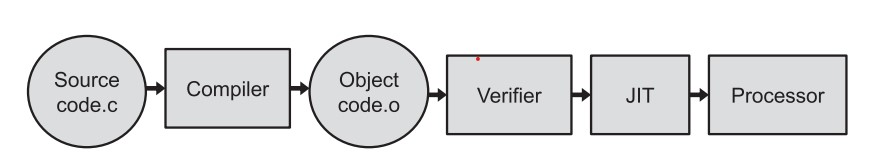
\includegraphics[width=0.9\columnwidth]{../LvHongtao/pic_1.jpg}
        \caption{eBPF运行原理示意图}
    \end{figure}
    \begin{enumerate}
        \item eBPF的程序可以直接通过C语言或RUST语言编写,
        经过专用的编译器编译成BPF字节码(bytecode)并提交给Verifier审核
        \item Verifier需要执行若干操作来确保收到的BPF program可以安全的在内核中运行,
        这些操作包括:
        \begin{enumerate}
            \item 限制BPF程序的总长度。
            \item 只允许出现固定轮数的循环。
            \item 只允许在程序结束时调用其他子程序作为延续。
            \item 只允许通过专用接口调用受限制的若干种系统调用。
            \item 程序的最坏运行时长不得超过某个值。
        \end{enumerate}
        在这些限制条件下,确保了BPF程序不会死循环,不会占用过多CPU时间,并且难以对OS造成损害。
        通过了verifier的程序会被送入JIT(JUST-IN-TIME Compiler)。
        \item JIT(JUST-IN-TIME Compiler)会将bytecode翻译成对应架构的二进制程序(如x86或arm的程序段)
        然后将此二进制程序放入专用内存空间存储和等待运行,使此程序的运行时拥有几乎原生的性能。
        \item 存储层面上,eBPF程序的代码段一经写入就会被设置为只读,防止其内容被篡改。
        eBPF程序也不能直接调用通用的内存空间进行本地数据的存储,其需要使用通过bpf helpers syscalls创建bpf map。
        内核态可以直接访问map,写入数据。用户态需要得到map's file descriptor,间接访问。
        BPF程序与用户态进程交互通过bpf map实现。
        
        \item 执行时,eBPF程序不允许主动的调用执行,只能通过BPF钩子(hook)被动的调用。
        通过在对应事件上注册BPF钩子即可在事件发生时调用对应程序。简单调用的场景例如:\\
        当任意系统调用发生时,调用某BPF程序记录系统调用的类型事件并写入系统日志;\\
        当接收到任意网络数据包时将所有类型为XXX的包发送给用户态程序进行分析。
    \end{enumerate}
    通过以上措施,BPF实现了灵活且安全的在内核态植入一些程序从而高效的实现了很多重要的功能。

    \item eBPF目前在网络分析、性能优化、负载调度等领域有众多应用,包括如下
    \begin{enumerate}
        \item 快速数据包处理,如控制分发操作(IoT)。
        \item 网络路由,子节点的路径管理(InKeV)。
        \item Container技术,将一套应用程序所需的执行环境打包起来。
        将BPF程序放进每个Container,对每个应用程序做出更强的管理(Cilium)。
        %%%%%%%%%%%%%% 这里填入后续补充的相关bpf项目 填个名目 详细内容写在后面 都加上引用 %%%%%%%%%%%
        \item bcc\cite{bcc2021}\\
        bcc即BPF Compiler Collection,是
        一个能高效编写内核追踪和管理程序的工具包。
        它是主要的BPF前端项目。
        用户能够为BPF编写C程序,或Python,lua,
        由BCC转化成BPF应用(借由LLVM生成字节码),是一种动态编译的方式。
        \item bpftrace\cite{bpftrace2021}\\
        构建于BPF和bcc之上的追踪工具。动态监测工具,
        同样用于与BPF进行交流。用户使用单行命令或编写程序获取目标进程的行为,
        或记录过程。
        \item libbpf\cite{BPFPort2020}\\
        libbpf目标是为了使得bpf程序像其它程序一样,编译好后,
        可以放在任何一台机器,任何一个kernel版本上运行。
        使用libbpf可以像编写普通用户态程序一样开发BPF程序,比BCC更精简快速。

        背景:有些BPF程序不需要获取内核数据结构,只是捕获系统调用,
        但是它们比较稀有;BPF提供了一些稳定接口,让部分结构具有统一性,
        但是十分有限。为了对付具有很强动态性的语境,BCC采用动态编译,
        但是为此付出了不简洁、存在错误率的代价。

        使用内核的BTF(BPF Type Format)信息可以实现结构定位,
        并且用它成功生成了一个巨大的头文件vmlinux.h,
        这个文件代替了特化的内核版本头文件,让程序具有到处运行的可能。

        在某些泛用条件下,BCC程序可以转化为libbpf程序。
        \item Falco\cite{Falco2021}\\
        应用反常行为监视工具。能持续性监视和侦测容器、应用、远程计算机、
        网络的行为,比如namespace的切换,敏感读写,执行shell。

        组成:
        \begin{enumerate}
            \item Userspace program,用户与Falco交流的命令行界面。
            \item Configuration,控制Falco的运作机制。
            \item Driver,一个获取系统调用并返回给用户态的工具,其中一个选择就是eBPF probe。
        \end{enumerate}
        \item Katran\cite{Katran2021}\\
        一个C++库/BPF程序,能够搭建高性能的layer 4负载均衡器。
        利用了XDP和BPF提供内核中的工具来进行快速包处理。
        Katran部署在Facebook的后端服务器上,
        它帮助Facebook提高了网络负载均衡的性能和可扩展性。

        XDP是一个内核组成,能进行快速包处理。
        \item Hbble\cite{Hbble2021}\\
        分布式网络安全保障和观测平台。构建于Cilium和BPF之上,
        能够深入获取信息,比如网络服务的交流频率,
        哪些网络服务被阻挡或者被服务集群外部访问,而借由BPF工具这些观测的开销很小。
        \item tracee\cite{tracee2021}\\
        实时的系统和应用追踪工具,能够分析、收集事件来探测可疑行为。
        它作为一个docker镜像来运作。使用go语言。

        其组成部分Tracee-eBPF用于事件收集。
        而libbpgo是一个帮助go编写BPF程序的库,使用了libbpf。
    \end{enumerate}
    具体的案例见后文相关工作部分

    %%%%%%%%%%%这段可以变成一个和bpf相关的引用,不要写在正文里了%%%%%%%%%%%%%%%%%%%%%
    %\item eBPF相关的源码在Linux源码的kernel/bpf中。不同linux版本的源码可以访问
    %\url{https://elixir.bootlin.com/linux/v4.20.17/source/kernel/bpf}
    %早期版本(如4.0.9)的bpf比后期的(如5.x.x)结构简单很多,代码量差距很大。也许可以先看以前的。
    

    %%%%%%%%%%% 可能适合放在总结部分 %%%%%%%%%%%%%%%%%%%%%
    %\item 我们的思考\\
    %JVM和eBPF的结构似乎很像,核心区别可能是JVM运行在用户态而eBPF运行在内核态,
    %同时eBPF出于安全原因有更多的安全限制,
    %也许可以通过学习JVM的相关知识来理解eBPF的实现。
    %或者可以参考JVM的结构让eBPF可以执行更多的功能。
    %\item 


\end{itemize}

\subsection{虚拟化技术}
虚拟化(技术)或虚拟技术(英语:Virtualization)是一种资源管理技术,
是将计算机的各种实体资源(CPU、内存、磁盘空间、网络适配器等),
予以抽象、转换后呈现出来并可供分割、组合为一个或多个电脑配置环境。
由此,打破实体结构间的不可切割的障碍,使用户可以比原本的配置更好的方式来应用这些电脑硬件资源。
这些资源的新虚拟部分是不受现有资源的架设方式,地域或物理配置所限制。
一般所指的虚拟化资源包括计算能力和资料存储。(wiki)
\begin{itemize}
    \item 虚拟机的分类
    \begin{enumerate}
        \item 完全虚拟化:虚拟机管理器将虚拟整个OS以满足任意软件的运行需求。
        一般的,其截获并筛选guestOS将要运行的指令,
        相对安全的指令将被提交给物理CPU直接运行,相对危险的指令(如修改系统时钟或修改中断寄存器)
        将被虚拟机管理器截获并且通过模拟运行结果的方式返回给guestOS。\\
        熟知的例子包括:QEMU、VMware等
        \item 部分虚拟化:虚拟机只针对特定应用程序进行虚拟,而不是虚拟整个操作系统。
        \item hypervisor模型:主机运行的OS直接负责执行虚拟化,VMM同时负责管理虚拟机和管理系统硬件
        \item host OS模型:VMM作为通用OS(如linux)的一个模块被加载,
        VMM通过请求系统调用来满足虚拟机的运行需求,VMM在OS视角来看类似于一个普通的进程。
        随着linux的虚拟化功能越来越多,他正在从Host模型发展为Hypervisor模型。
        \item 混合模型:VMM作为最底层调度硬件,
        但是额外运行了一个虚拟的操作系统来执行IO的适配,
        通过这种模式,VMM开发者不必编写大量代码适配各种复杂的硬件,减轻了开发难度。
        但相对的guestOS的请求需要多次转发才能得到满足,影响了性能。
    \end{enumerate}
    \item 虚拟机的实现结构
    \begin{enumerate}
        \item hypervisor模型:主机运行的OS直接负责执行虚拟化,VMM同时负责管理虚拟机和管理系统硬件
        \item host OS模型:VMM作为通用OS(如linux)的一个模块被加载,
        VMM通过请求系统调用来满足虚拟机的运行需求,VMM在OS视角来看类似于一个普通的进程。
        随着linux的虚拟化功能越来越多,他正在从Host模型发展为Hypervisor模型。
        \item 混合模型:VMM作为最底层调度硬件,
        但是额外运行了一个虚拟的操作系统来执行IO的适配,
        通过这种模式,VMM开发者不必编写大量代码适配各种复杂的硬件,减轻了开发难度。
        但相对的guestOS的请求需要多次转发才能得到满足,影响了性能。
    \end{enumerate}
    \item 虚拟化可以使用的两种特殊场景
    \begin{enumerate}
        \item 沙盒:为了保护宿主OS不被恶意进程破坏而制作出来的隔离运行环境。
        \item 容器:为了追求部署的便利和运行的效率而制作出来的高效运行环境。
    \end{enumerate}
\end{itemize}

\subsection{沙盒}
沙盒(英语:sandbox,又译为沙箱)是一种安全机制,为运行中的程序提供的隔离环境。
通常是作为一些来源不可信、具破坏力或无法判定程序意图的程序提供实验之用。
沙盒通常严格控制其中的程序所能访问的资源,比如,沙盒可以提供用后即回收的磁盘及内存空间。
在沙盒中,网络访问、对真实系统的访问、对输入设备的读取通常被禁止或是严格限制。
从这个角度来说,沙盒属于虚拟化的一种。
沙盒中的所有改动对操作系统不会造成任何损失。
通常,这种技术被计算机技术人员广泛用于测试可能带毒的程序或是其他的恶意代码。(wiki)

\begin{enumerate}

\item 传统上为了实现沙盒可以使用如下的若干种方式
\begin{itemize}
    \item 软件监狱(Jail):限制网络访问、受限的文件系统namespace。
    \item 基于规则的执行:通过系统安全机制,按照一系列预设规则给用户及程序分配一定的访问权限,
    完全控制程序的启动、代码注入及网络访问[5]。也可控制程序对于文件、注册表的访问。
    在这样的环境中,病毒木马感染系统的几率将会减小。
    Linux中,安全增强式Linux和AppArmor正使用了这种策略
    \item 虚拟机:模拟一个完整的宿主系统,可以如运行于真实硬件一般运行虚拟的操作系统(客户系统)。
    客户系统只能通过模拟器访问宿主的资源,因此可算作一种沙盒。
    \item 在线判题系统:用于编程竞赛中的程序测试。
    \item 安全计算模式(seccomp):Linux内核内置的一个沙盒。
    启用后,seccomp仅允许write()、read()、exit()和sigreturn()这几个系统调用。(后文将会详细介绍此技术)

\end{itemize}

\item 近年来计算机安全需求不断升级,又出现了很多新兴的沙盒技术
\begin{itemize}
    \item unikernel:给应用带上自己的核,开销较小并且难以被攻击,其缺点在于需要单独设计对应的应用。
    \item MicroVM: 运行另一个剪裁过的内核并将其暴露给应用程序,恶意进程将难以同时攻破两个OS的安全措施。
    \item 进程虚拟化:利用软件模拟出linux运行环境,能够强化沙盒的安全性。(其安利gvisor将在后文被详细分析)
\end{itemize}

\item linux对沙盒技术的支持主要包括以下三个工具
\begin{itemize}
    \item \textbf{seccomp}\\
    \href{https://en.wikipedia.org/wiki/Seccomp}{seccomp}介绍。
    传统seccomp可以让某个进程进入安全模式,并且阻止其调用所有除了exit(),
    sigreturn(),read(),write()外的所有对file descriptor (FD) 的调用,
    一旦发现此类调用就立即kill进程。后来引入bpf后形成了seccomp/bpf,可以更灵活的设置拦截的规则。
    seccomp使用的是cBPF\cite{calavera2019linux},
    seccomp/bpf以bpf程序的形式定义了一个系统调用的白名单,
    被seccomp/bpf约束的进程可以自由的请求白名单内的系统调用,
    但一旦进程发出了不许可的指令,它将会被立刻终结。
    这种沙盒工具只是利用BPF限制了系统调用,沙盒内外的程序运行环境没有其他区别。
    \cite{2020SandboxLinux}

    \item \textbf{Cgroups}\\
    \href{https://en.wikipedia.org/wiki/Cgroups}{Cgroups}介绍。
    其主要支持四个功能:
    \begin{enumerate}
        \item 限制某些groups的资源使用量(包括CPU,IO,内存等)
        \item 调整优先级,使某些group可以分配到更多的资源
        \item 记录某些group的资源使用量
        \item 控制某些group的运行,具体的可以冻结,快照,重启。
    \end{enumerate}

    \item \textbf{Linux Namespace}\\
    Linux的Namespace机制是一种资源隔离方案。它将 Linux 的全局资源,
    划分为 namespace 范围内的资源,而且不同 namespace 间的资源彼此透明,
    不同 namespace 里的进程无法感知到其它 namespace 里面的进程和资源。
    但是namespace机制有缺陷。
    \begin{enumerate}
        % \item Non-namespace-aware system call interface facilitates
        % the adversary to compromise applications running in containers 
        % and further exploit kernel vulnerabilities to elevate privileges, 
        % bypass access control policy enforcement, 
        % and escape isolation mechanisms.
        \item Non-namespace-aware system调用接口可帮助对手破坏容器中运行的应用程序,
        并进一步利用内核漏洞来提升权限,绕过访问控制策略并逃过隔离机制。\cite{2019Practical}
        \item 某种沙盒使用的安全方案\cite{2019Practical}:
        用自动测试锁定一个container中程序的系统调用。
        然后在实际运行中阻止非锁定的任何系统调用。但是锁定系统调用不算特别理想。
        程序调用的是API,间接执行系统调用,不容易直接发现。
        有的程序将近一半的可能系统调用都没被发掘。对于开发者来说,
        可以加入自己的测试过程来辅助锁定。
    \end{enumerate}

\end{itemize}

\end{enumerate}

\subsection{容器}
操作系统层虚拟化(英语:Operating system–level virtualization),亦称容器化(英语:Containerization),
是一种虚拟化技术,这种技术将操作系统内核虚拟化,可以允许用户空间软件实例(instances)被分割成几个独立的单元,
在内核中运行,而不是只有一个单一实例运行。

这个软件实例,也被称为是一个容器(containers),虚拟引擎(Virtualization engine),
虚拟专用服务器(virtual private servers)或是 jails。对每个行程的拥有者与用户来说,
他们使用的服务器程序,看起来就像是自己专用的。

操作系统层虚拟化之后,可以实现软件的即时迁移(Live migration),使一个软件容器中的实例,
即时移动到另一个操作系统下,再重新运行起来。但是在这种技术下,软件即时迁移,只能在同样的操作系统下进行。

在类Unix操作系统中,这个技术最早起源于标准的chroot机制,再进一步演化而成。
除了将软件独立化的机制之外,内核通常也提供资源管理功能,使得单一软件容器在运作时,
对于其他软件容器的造成的交互影响最小化。

相对于传统的虚拟化(Virtualization),容器化的优势在于占用服务器空间少,
通常几秒内即可引导。同时容器的弹性可以在资源需求增加时瞬时复制增容,
在资源需求减小时释放空间以供其他用户使用。由于在同一台服务器上的容器实例共享同一个系统内核,
因此在运行上不会存在实例与主机操作系统争夺RAM的问题发生,从而能够保证实例的性能。(wiki)
\subsubsection{Docker}

% Docker调研

\section{立项依据}

本项目旨在实现一种兼有安全性与运行效率的沙盒架构。提高沙盒的安全性与运行效率是当今计算机界的重要课题,
但当前现有的工作或在安全性上存在漏洞,或在性能上无法让人满意,难以同时在这两个方向上达到较好的水平。
本项目突破了用户态与内核态二选一的固有思维方式,将eBPF技术引入这一领域,
尝试利用eBPF这一新兴技术实现安全性和性能的最大化。eBPF技术可以在用户态进程的引导下在内核态运行特定代码段,
从而此框架可以实现用户态的灵活性和内核态的高效。近年来,这一框架的潜力正不断被业界挖掘出来,
基于eBPF的各种功能不断的被实现,众多传统模块也已经在eBPF框架下实现了升级。
我们的项目也将借助eBPF架构的优点,借鉴同类eBPF项目的经验,解决传统沙盒的各种弊端,
实现对传统沙盒的全方位优化。

\section{项目重要性}

传统的沙盒/容器技术存在着实现在内核或者用户态的选择问题。
内核态实现的沙盒/容器技术功能存在着更新和修改困难的问题,
每次对沙盒代码的修改和升级都需要重新对此内核模块进行加载。
而且在内核中实现这类功能也可能会给内核增加潜在的攻击点,
或者因为潜在的错误使内核稳定性降低。而在用户态实现的沙盒/容器技术虽然可以实现简单的更新和修改,
且不易影响内核的正常运行,但是由于此类应用经常需要一些底层的系统操作支持,
因此会存在大量的用户态到内核态的切换,带来严重的性能问题。
综上,寻求一种兼有内核态与用户态优点的解决方案十分重要。

将eBPF程序引入此领域可以一举解决很多现有问题,eBPF程序运行在内核态,
因此其运行性能相当之高,同时其实现机制可以确保此引入到内核的程序难以对内核其他功能造成威胁,
确保内核运行的安全。eBPF程序的修改可以在用户态引导进行,其基于hook的调用机制甚至可以支持热升级,
能实现在不中断服务的情况下升级程序。

\section{相关工作}

\subsection{MBOX}
MBOX是一个为非root用户提供的沙盒环境,主要面对filesystem进行保护。

在与MBOX有关的一篇论文\cite{180196}中,
详细介绍了此沙盒面对的使用场景与其解决方案,
此沙盒使用了上文提到的seccomp-bpf作为工具增强其安全性。

\begin{itemize}
    \item 此沙盒面对的使用场景如下:
    \begin{enumerate}
        \item 为非管理员用户构造虚拟的root权限,便于这类用户执行一些特殊的任务。
        例如vlab提供的fakeroot即为此类应用。
        \item 安全地运行不可信的二进制文件,可以用于分析潜在的恶意程序或病毒。
        \item 为文件系统提供检查点(check point)。
        当用户需要处理危险的文件的时候,
        传统上一旦文件出现错误就需要使用专用工具修复文件系统。
        使用MBOX则可以在开始处理前把运行环境转移到虚拟的文件系统中,
        这样在发生错误后可以提取sandbox中剩余的错误信息,
        并且可以正常的时候原理的文件系统,
        如果运行成功了也可以直接把sandbox的系统与原文件系统合并(听起来很像git)。
        \item 使用MBOX,用户可以简单的构建开发环境,构建过程只需要将配置好的开发环境整体移植到沙盒内即可完成。
        \item 细化文件权限管理,通用os如linux中用户建立的进程有权限访问用户的所有个人文件,
        使用MBOX可以使特定用户进程只能访问必须的文件,保护了其他文件。
    \end{enumerate}
    \item 其大致上的实现原理如下:
    \begin{enumerate}
        \item 给文件系统增加了一个private layer,位于原生文件系统的上层,
        每个sandbox会对应生成一个MBOX文件系统,用于服务沙盒中的进程。
        此文件系统的储存结构从原生文件系统的角度来看只是普通的目录,
        但是沙盒中的程序必须通过MBOX获得文件服务。
        \item 虚拟文件系统中的文件变动不会实时更新到host文件系统,
        但是host文件系统中的变动可以实时同步到虚拟文件系统中,
        当两个系统出现冲突的时候由用户决定保留哪一个版本。
        \item 使用了\textbf{seccomp-bpf}和
        \textbf{ptrace}干预系统调用并且实现fakeroot。具体的,其作为过滤器来干预沙盒中进程的syscall,
        如限制某进程对socket的调用。
        \item 其对sefccomp-bpf的使用与我们的设想相同,
        将每个syscall的进入调用挂在某个bpf程序上,
        bpf程序接受syscall的类型,进程的属性等信息,计算是否有相应权限。
    \end{enumerate}
    
\end{itemize}

\subsection{gVisor}
gVisor 是一款新型沙箱解决方案,其能够为容器提供安全的隔离措施,
同时继续保持远优于虚拟机的轻量化特性。gVisor能够与Docker及Kubernetes实现集成,
从而在生产环境中更轻松地建立起沙箱化容器系统。

gVisor能够在保证轻量化优势的同时,提供与虚拟机类似的隔离效果。
gVisor的核心为一套运行非特权普通进程的内核,且支持大多数Linux系统调用。
该内核使用Go编写,这主要是考虑到Go语言拥有良好的内存管理机制与类型安全性。
与在虚拟机当中一样,gVisor沙箱中运行的应用程序也将获得自己的内核与一组虚拟设备
——这一点与主机及其它沙箱方案有所区别。(gVisor主页)

\subsubsection{gVisor的结构与问题}

论文\cite{234857}提出来了如下观点:

\begin{enumerate}
    \item 传统来说,hyperviser模式的虚拟化容器有着更好的安全性,
    但是难以保证性能。hostOS结构的容器(如docker)
    的性能更好是由于其运行的若干的虚拟机通过一个统一的完善的通用OS来调度各类资源。
    但是由于hostOS结构中hostOS本身没有运行在容器中,
    其本身的内核bug容易成为被攻击的目标。 
    (详细分析见此文\href{https://opensource.com/business/14/7/docker-security-selinux}
    {Are Docker containers really secure?}\cite{DanielJDocker}) 
    
    \item gviser的存在一些性能问题,如打开关闭文件比传统容器慢了216倍,
    其他操作也普遍慢了很多(2倍到11倍)。
    \item gVisor支持OCI(Open Container Initiative),
    因此docker用户可以自己配置使用默认引擎,runc或者gvisor作为runtime engine。
    \item gVisor结构如下 guestApp-Sentry( VMM+guestOS(linux) )-hostOS,
    多层结构确保程序难以同时攻克每一层的安全缺陷,损害hostOS的安全。
    sentry提供两种工作模式,第一种模式中其追踪并且翻译gusetAPP的系统调用,
    第二种模式中其更像是虚拟机中工作的guestOS,直接服务guestAPP。
    \item gVisor为guestAPP提供了211个syscall(标准linux提供了319种),
    gVisor只需要向hostOS请求55种syscall,
    这些syscall的种类都是通过seccomp技术限制和约束的,
    当sentry被guestAPP劫持并且申请了超出允许范围的syscall时,
    seccomp过滤器会把gVisor杀死从而确保hostOS的安全。
    诸如OPEN和SOCKET这样的操作被设计者认为是极端危险的,
    因此没有被列入许可的syscall,这两个功能是通过复杂的结构设计出来的,
    从而保证可以在不调用hostOS的对应syscall的前提下安全的为guestAPP提供服务。
    这就是为什么gVisor的文件性能如此差。
    \item gVisor对文件服务的实现:
    \begin{itemize}
        \item sentry实现了若干个不同的内置文件系统来尽可能满足guestAPP的请求。
        \item 当有必要读取hostOS文件系统时,他调用Gofer来替其进行文件访问,
        访问结果(文件句柄)通过一个P9 Channel返回给sentry(进程间通讯),
        
        \item sentry得到句柄后需要进行用户态到内核态的转化和上下文切换才能进行读取。
    \end{itemize}
    此过程导致了gvisor在文件访问效率上的低速,但带来了可靠的安全性。
    
    \item 本文提出了若干种对此类容器进行性能测试的方法。
    %\item 其他进程如何实现劫持沙盒管理程序的权限(如open函数),或许能体现BPF的优势,
    % 需要调研现有安全漏洞的形式。
\end{enumerate}


\bibliography{../paper.bib}
\bibliographystyle{ieeetr}

\end{document}